\documentclass{thesis-tobias}

%% Set up the bibliography
\usepackage{biblatex}
\addbibresource{report.bib}

%% Additional packages and commands
\usepackage{parskip}
\setlist{itemsep=-2pt} % Reducing white space in lists slightly
\renewcommand{\deg}{\si{\degree}\xspace} % Use \deg easily, everywhere

%% ----------------------------------------------------------------------
%%    Begin of document + Frontmatter (Roman page numbering)
%% ----------------------------------------------------------------------
\setenumerate[2]{label=\alph*.}
\newcolumntype{C}[1]{>{\centering\arraybackslash}p{#1}}

\usepackage{amssymb}% http://ctan.org/pkg/amssymb
\usepackage{pifont}% http://ctan.org/pkg/pifont
\newcommand{\cmark}{\ding{51}}%
\newcommand{\xmark}{\ding{55}}%

\begin{document}

\frontmatter

%% Define the main parameters
\title{title}
\subtitle{subtitle}
\author{someone}

\LatestVersion{1}

\subject{Project DragonFly} % Cover only
\affiliation{Inholland University of Applied Sciences Delft} % Cover only
\coverimage{figures/Motor1.jpg} % Aspect ratio of 2:3 (portrait) recommended
\definecolor{title}{HTML}{4884d6} % Color for cover title

\makecover

\begin{titlepage}

\begin{center}

%% Print the title
{\makeatletter
\largetitlestyle\fontsize{45}{45}\selectfont\@title
\makeatother}

%% Print the subtitle
{\makeatletter
\ifdefvoid{\@subtitle}{}{\bigskip\titlestyle\fontsize{20}{20}\selectfont\@subtitle}
\makeatother}

\bigskip
\bigskip

by

\bigskip
\bigskip

%% Print the name of the author
{\makeatletter
\largetitlestyle\fontsize{25}{25}\selectfont\@author
\makeatother}

\bigskip
\bigskip

%% Print table with names and student numbers

\vfill

%% Print some more information at the bottom
\begin{tabular}{ll}
    Last updated: & \today 
\end{tabular}

\bigskip
\bigskip

%% Add a source and description for the cover and optional attribution for the template
\begin{tabular}{p{15mm}p{10cm}}
    Cover: & Dragonfly PH-HBR, Teuge Airport (TW. Kroes) \\
    % Feel free to remove the following attribution, it is not required - still appreciated :-)
    Style: & TU Delft Report Style, with modifications
\end{tabular}

\end{center}

%% Insert the Inholland logo at the bottom of the page
\begin{tikzpicture}[remember picture, overlay]
    \node[above=10mm] at (current page.south) {%
        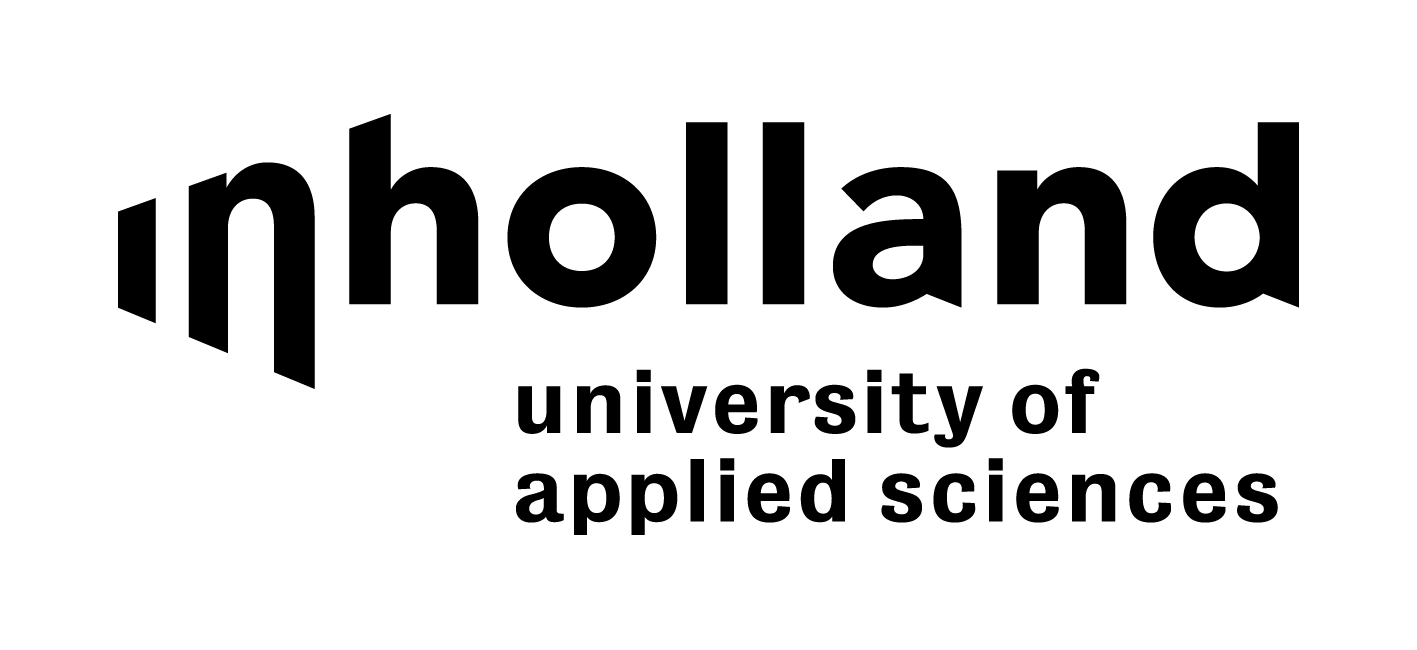
\includegraphics[width=0.35\linewidth]{figures/Inholland_University_black.png}
    };
\end{tikzpicture}

\end{titlepage}

\chapter*{Preface}

\textbf{This document is classified as 'confidential.'} This means that its access is limited exclusively to the members of the Project DragonFly team and Saluqi Motors. The contents of this document contain sensitive and confidential information that is intended solely for internal use.

\vspace*{\fill}

\emph{The table below indicates the original issue and the revisions, which were made from the original release to this date.}

\section*{Revisions}
\begin{center}
\begin{longtable}{p{2cm}p{2.5cm}p{2.5cm}p{2.5cm}p{4cm}}
	\toprule
	Designation & Implemented By & Revision Date & Affected pages &  Reason \\
	\midrule\endhead % Add Latin symbols alphabetically here:
	$0.1$ & name & date & All & Initial Document\\
	\bottomrule
	\bottomrule
\end{longtable}
\end{center}

\vspace*{\fill}
\begin{flushright}
{\makeatletter\itshape
    \@author \\
    Delft, \monthname{} \the\year{}
\makeatother}
\end{flushright}
 

\tableofcontents
%\listoffigures
%\listoftables

%\chapter*{Nomenclature}
\addcontentsline{toc}{chapter}{Nomenclature}

\section*{Abbreviations}

\begin{longtable}{p{2.5cm}p{8cm}}
    \toprule
    Abbreviation & Definition \\
    \midrule\endhead % Add abbreviations alphabetically here:
    DF  & Dragonfly \\
    BMS & Battery Management System\\
    AWG & American Wire Gauge\\
    BR & Business Requirement \\
    SP & Requirement specifier \\
    FR & Functional Requirement \\ 
    PR & Performance Requirement \\
    \bottomrule
\end{longtable}

\section*{Symbols}

\begin{longtable}{p{2.5cm}p{8cm}p{2.5cm}}
    \toprule
    Symbol & Definition & Unit \\
    \midrule\endhead % Add Latin symbols alphabetically here:
    $d_t$ & Throat diameter & [mm] \\
        ... \\
    \midrule % Add Greek symbols alphabetically here:
    $\rho$ & Density & [kg/m$^3$] \\
    ... \\
    \bottomrule
\end{longtable}


%% ----------------------------------------------------------------------
%%    Mainmatter (Arabic page numbering)
%% ----------------------------------------------------------------------

\mainmatter

\chapter{introduction}

\section{Purpose}
\section{Scope}
\section{Objectives}



\chapter{System Overview}

\section{Description of the System}
\section{ System Architecture}
\section{Interfaces}
\section{Regulatory Compliance}






\chapter{Test Strategy}


\section{ Testing Levels}
\section{ Testing Types}
\section{Entry and Exit Criteria}
\section{ Test Deliverables}
\section{Test Environment}
\section{Hardware}
\section{Software}
\section{Test Schedule}
\section{Risks and Contingencies}









\input{mainmatter/TestCases}
\chapter{Test Excecution}

\section{Test Execution Schedule}
\section{Test Execution Team}
\section{Test Execution Procedure}
\section{Test Data Preparation}
\section{Logging and Tracking Defects}
\section{Regression Testing}
\section{Performance Testing}








\chapter{Test Reporting}

\section{Test Summary Report}
\section{Defect Summary Report}
\section{Traceability Matrix}
\section{Metrics and Measurements}




\chapter{Test Sign off}

\section{ Criteria for Test Completion}
\section{Approval Signatures}
\section{Approval Signatures}


%% Prevent urls running into margins in bibliography
\setcounter{biburlnumpenalty}{7000}
\setcounter{biburllcpenalty}{7000}
\setcounter{biburlucpenalty}{7000}

%% Add bibliography
\printbibliography[heading=bibintoc,title=References]

%% ----------------------------------------------------------------------
%%    Appendix (Letters for chapters)
%% ----------------------------------------------------------------------

\appendix

%\chapter{Source Code }
%\label{chapter:title}

\emph{Adding source code to your report/thesis is supported with the package {\normalfont\texttt{listings}}. An example can be found below. Files can be added using {\normalfont\texttt{\textbackslash lstinputlisting[language=<language>]\{<filename>\}}}.}

\begin{lstlisting}[language=Python]
"""
ISA Calculator: import the function, specify the height and it will return a
list in the following format: [Temperature,Density,Pressure,Speed of Sound].
Note that there is no check to see if the maximum altitude is reached.
"""

import math
g0 = 9.80665
R = 287.0
layer1 = [0, 288.15, 101325.0]
alt = [0,11000,20000,32000,47000,51000,71000,86000]
a = [-.0065,0,.0010,.0028,0,-.0028,-.0020]

def atmosphere(h):
    for i in range(0,len(alt)-1):
        if h >= alt[i]:
            layer0 = layer1[:]
            layer1[0] = min(h,alt[i+1])
            if a[i] != 0:
                layer1[1] = layer0[1] + a[i]*(layer1[0]-layer0[0])
                layer1[2] = layer0[2] * (layer1[1]/layer0[1])**(-g0/(a[i]*R))
            else:
                layer1[2] = layer0[2]*math.exp((-g0/(R*layer1[1]))*(layer1[0]-layer0[0]))
    return [layer1[1],layer1[2]/(R*layer1[1]),layer1[2],math.sqrt(1.4*R*layer1[1])]
\end{lstlisting}


\end{document}
